\pdfoutput=1
\documentclass[11pt]{article}

\usepackage[margin=1in]{geometry}
\usepackage{times}
\usepackage{graphicx}
\usepackage{booktabs}
\usepackage{placeins}
\usepackage{array}
\usepackage{float}
\usepackage{amsmath}
\usepackage{amssymb}
\usepackage{enumitem}
\usepackage[round]{natbib}
\usepackage[hidelinks]{hyperref}

\graphicspath{{figures/}}

\title{RAMP: A Multi-Stage Safety Classifier for Accumulating Prompt, Internal, Output, and Session Risk Signals}

\author{
Ratnaditya J.\\
RAMP Reference Implementation\\
\texttt{https://github.com/Ratnaditya-J/RAMP}
}

\date{Research draft}

\begin{document}
\maketitle

\begin{abstract}
Safety classification for large language model (LLM) and agent systems is commonly framed as a
single prompt- or response-level decision. Real deployments, however, expose staged evidence:
the user prompt, model-internal representations, generated output, multi-turn session history, and
proposed tool actions. We present RAMP, a reference implementation and research design for a
multi-stage safety classifier that accumulates such evidence into a versioned risk state. The
current RAMP reference implementation implements prompt classification, GPT-OSS input-embedding
proximity, GPT-OSS activation probes, generated-output classification, session classification, and
tool/action gating. On the current 448-row human-reviewed hard-case prompt set, cross-fitted,
leakage-free split-stability calibration selects prompt+embedding as the primary input-side runtime
policy: prompt weight 0.80, input-embedding weight 0.20, activation weight 0.00, and threshold 0.50.
This policy reaches mean AUROC 0.9627, mean recall 0.9608, and mean false-positive rate 0.1085
across 30 deterministic reviewed-label splits, compared with prompt-only AUROC 0.9458 and false
positive rate 0.1238. Activation, output classification, and full-transcript session scoring are
useful as research, audit, post-generation, or escalation evidence, but they do not yet justify
positive runtime blocking weight under the leakage-free protocol. The main
finding is therefore not that every signal improves runtime blocking, but that a staged reference design can
make signal value, negative results, and provenance explicit enough for reproducible safety research.
\end{abstract}

\section{Introduction}

Safety filters for LLM systems are often evaluated as one-shot classifiers: given a prompt or model
response, return safe or unsafe. This framing is useful but incomplete. Interactive and agentic
systems produce additional evidence over time: multiple prompts in a session, internal model states,
generated responses, tool calls, and action arguments. A prompt may look ambiguous in isolation but
become high risk after session context accumulates; a generated answer may be safer or less safe
than the original prompt suggested; an internal activation pattern may separate hard benign
near-neighbors from harmful requests. These observations motivate a multi-stage classifier rather
than a single-stage guard.

RAMP tests this design hypothesis. It is not proposed as a replacement for existing safety
classifiers such as Qwen3Guard, Llama Guard, WildGuard, or commercial moderation APIs. Instead, RAMP
treats those classifiers as one stage in a broader evidence pipeline. Each stage emits a versioned
score, label, confidence, metadata, and provenance record. A fusion policy then combines the
available evidence and records which signals were decisive, missing, ignored, or reserved for audit.

This paper reports the current research result. The RAMP reference implementation is
feature-complete, but not production-grade or paper-final. Its strongest current evidence supports a
prompt+embedding input-side runtime core. Activation, output, and session scoring currently serve
audit, research, or escalation roles. We include these limited and negative results because they are
central to the contribution: RAMP provides a disciplined way to test whether signals earn runtime
weight instead of assuming every added stage should improve decisions.

The contributions are:
\begin{itemize}[leftmargin=*]
\item A versioned multi-stage safety-classifier reference design spanning prompt, embedding,
activation, output, session, and tool/action evidence.
\item A GPT-OSS-based internal-signal path that distinguishes input embeddings from hidden-state
activations and evaluates them separately.
\item A reviewed-label calibration protocol that freezes weights by cross-fitted split-stability
rather than manual preference or in-sample probe performance.
\item A consolidated evidence package showing which signals currently earn runtime weight and
which remain audit/escalation signals.
\end{itemize}

\section{Related Work}

\paragraph{Guard classifiers.}
Recent open guard models provide prompt- and response-level safety classification. Llama Guard
frames input-output safeguarding for human-AI conversations \citep{llamaguard2023}. WildGuard
contributes an open moderation model and training mixture for prompt/response safety
\citep{wildguard2024}. Qwen3Guard provides generative safety classification models used in our
prompt and output scoring experiments \citep{qwen3guard2025}. These systems motivate RAMP's
front-door and post-generation classifier stages.

\paragraph{Safety benchmarks and datasets.}
RAMP uses benchmark-derived rows for representation extraction and targeted review. HarmBench
provides a standardized harmful-behavior benchmark for automated red teaming
\citep{harmbench2024}. BeaverTails supplies safety-alignment data for helpfulness and harmlessness
analysis \citep{beavertails2023}. R-Judge, MHJ, and SafeDialBench motivate multi-turn/session
evaluation \citep{rjudge2024,mhj2024,safedialbench2025}. Because these sources have different label
semantics and class balance, RAMP treats them as distinct evidence sources rather than a single
homogeneous benchmark.

\paragraph{Internal representations and open-weight targets.}
RAMP separates input embeddings from activations. Input embeddings are the token-embedding vectors
produced before transformer-layer computation; activations are hidden states from later layers. For
current extraction, both are taken from the open-weight GPT-OSS path \citep{gptoss2025}, which
keeps the representation source tied to an instrumentable target model.

\paragraph{Policy and constitutional classifiers.}
Constitutional or policy-driven classifiers demonstrate that safety decisions can be encoded as
explicit policies with calibrated model judgments \citep{constitutionalclassifiers2025}. RAMP is
compatible with this direction but focuses on accumulating heterogeneous evidence and preserving
stage-level provenance.

\clearpage

\section{RAMP Method}

\subsection{Staged Evidence}

Figure~\ref{fig:pipeline} summarizes the RAMP pipeline.

\begin{figure}[H]
\centering
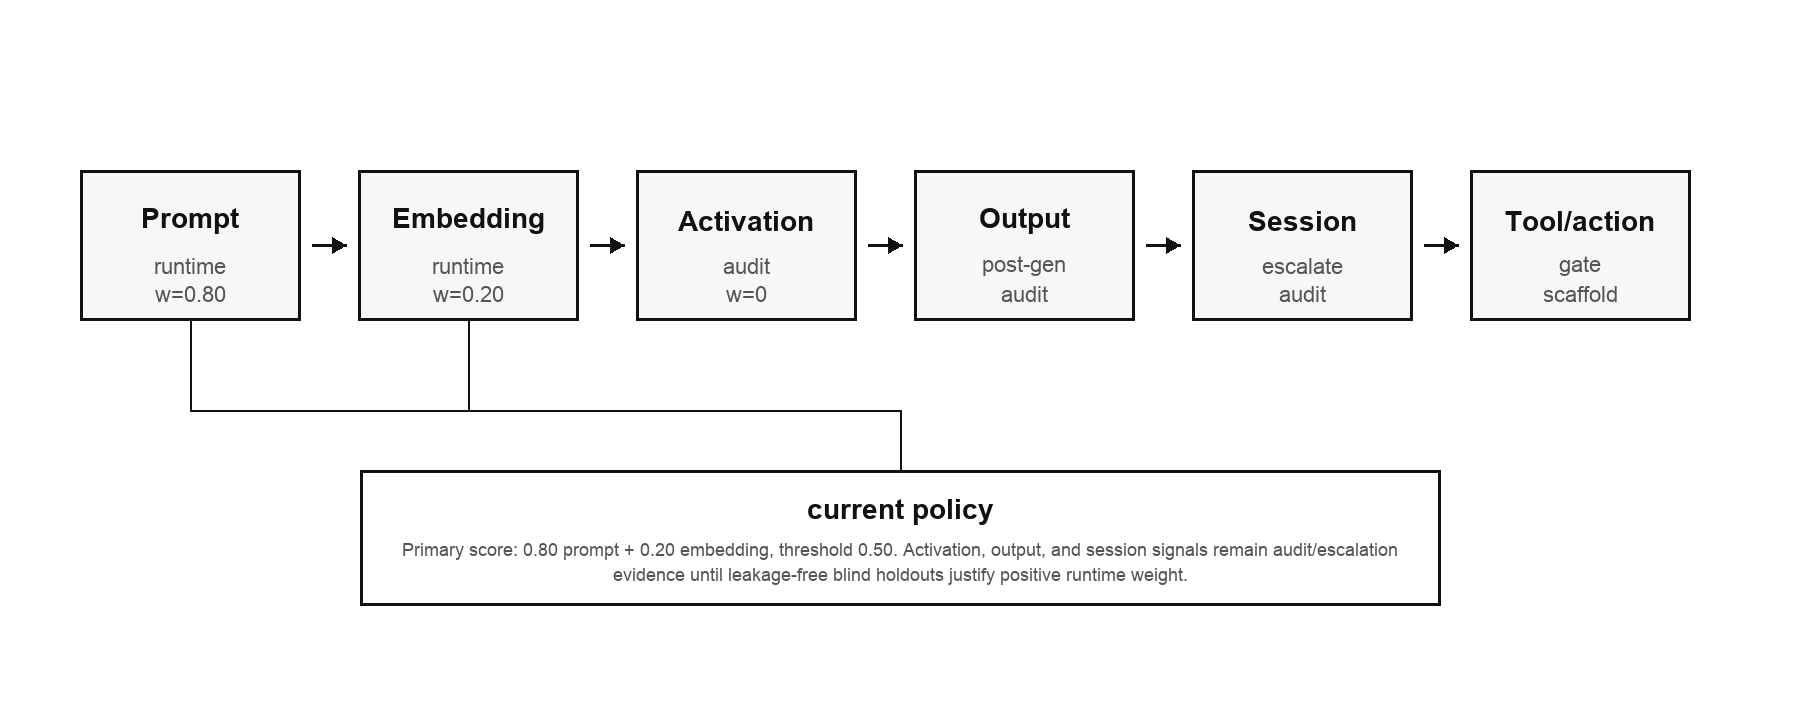
\includegraphics[width=0.84\textwidth]{ramp_pipeline.png}
\caption{RAMP accumulates staged evidence. The current frozen input-side runtime core uses prompt
and embedding scores. Activation, output, and session signals are retained as audit/escalation
evidence until leakage-free blind holdouts justify positive runtime weight.}
\label{fig:pipeline}
\end{figure}

The stages are:
\begin{enumerate}[leftmargin=*]
\item \textbf{Prompt classifier}: Qwen3Guard scores the incoming prompt.
\item \textbf{Input-embedding proximity}: GPT-OSS input embeddings are compared with harmful and
benign near-neighbor centroids.
\item \textbf{Activation probe}: a linear probe scores GPT-OSS hidden-state activations.
\item \textbf{Output classifier}: generated responses are scored after generation.
\item \textbf{Session classifier}: compact session evidence and full transcript evidence are scored
for multi-turn risk.
\item \textbf{Tool/action gate}: proposed tool calls and action arguments are checked by a
deterministic reference gate.
\end{enumerate}

\subsection{Fusion Policy}

Let $s_p$ be the prompt risk score, $s_a$ the activation probability, and $s_e$ the embedding prior.
The frozen input-side runtime score is
\begin{equation}
  s_{\mathrm{RAMP}} = 0.80 s_p + 0.20 s_e + 0.00 s_a.
\end{equation}
The selected operating threshold is 0.50. This score is wrapped by severity-aware floors: if the
prompt classifier marks a high-severity unsafe category, the final risk can be raised to a
configured minimum. The floor is a policy guardrail around calibrated fusion, not another learned
weight.

The threshold is not hand tuned. In each of 30 deterministic stratified reviewed-label splits, we
calibrate candidate weights and thresholds on the calibration half by grid search, using 0.05
weight steps and 0.01 threshold steps. Activation probes are retrained inside each split: calibration
rows receive out-of-fold activation predictions, and holdout rows receive predictions from a probe
trained only on that split's calibration rows. The selection objective orders candidates by F1,
accuracy, recall, false-positive rate, and AUROC on the calibration split. The reported weights and
threshold are the most common selected prompt+embedding configuration across splits. We treat this
as a stability-selected research operating point, not as a universal deployment cutoff.

The multi-stage policy artifact also defines non-primary roles. Output scoring is a post-generation
audit signal. Session scoring is a calibrated escalation/audit signal. Tool/action gating is a
deterministic reference gate pending benchmark validation.

\begin{table}[H]
\centering
\small
\newcolumntype{L}[1]{>{\raggedright\arraybackslash}p{#1}}
\begin{tabular}{L{0.17\textwidth}L{0.27\textwidth}L{0.20\textwidth}L{0.24\textwidth}}
\toprule
Signal & Final construction & Current role & Selection evidence \\
\midrule
Prompt classifier & Qwen3Guard prompt-risk score & Positive runtime signal & Reviewed labels
showed useful ranking after noisy benchmark labels were separated. \\
Embedding proximity & GPT-OSS input embeddings against harmful and benign centroids &
Positive runtime signal, pending blind holdout & Improves AUROC, F1, accuracy, and FPR over
prompt-only under cross-fitted reviewed split stability. \\
Activation probe & Linear probe over GPT-OSS layer-19 hidden states & Audit/research signal,
runtime weight 0 & In-sample activation results were optimistic; leakage-free cross-fitting did
not improve the selected runtime tradeoff over prompt+embedding. \\
Output classifier & Qwen3Guard score over generated response & Post-generation audit signal &
Output-inclusive fusion did not improve the best input-side result. \\
Session classifier & Compact evidence and full transcript evidence & Escalation/audit signal &
Full transcript catches misses; compact state is lossy and max fusion raises FPR. \\
Tool/action gate & Deterministic check over proposed tool arguments & Reference gate & Implemented
pattern; dedicated benchmark still pending. \\
\bottomrule
\end{tabular}
\caption{Signal construction and disposition in the current RAMP reference implementation. This
table separates implementation status from runtime weight: a signal can be implemented and useful
without earning positive blocking weight.}
\label{tab:signals}
\end{table}

\section{Data and Artifacts}

Table~\ref{tab:data} lists the major datasets and artifacts used in the current study. Large generated artifacts
are intentionally not committed to Git; the repository records their paths, summaries, and
provenance in the artifact registry.

\begin{table}[H]
\centering
\begin{tabular}{llr}
\toprule
Artifact or dataset & Purpose & Size \\
\midrule
Benchmark-derived corpus & embedding and activation extraction & 27,718 rows \\
Reviewed prompt set & prompt/internal fusion calibration & 448 binary reviewed rows \\
Output eval set & prompt/response output-classifier calibration & 134 rows \\
R-Judge & labeled multi-turn session evaluation & 555 sessions \\
MHJ & unsafe-only multi-turn jailbreak stress test & 496 sessions \\
SafeDialBench & session mining and future review & 4,053 sessions \\
\bottomrule
\end{tabular}
\caption{RAMP data sources. The corpora are used for different experimental questions and are not
treated as a single merged benchmark.}
\label{tab:data}
\end{table}

\section{Experiments}

The experiments are organized by signal family and by the decision each signal must earn. We do not
assume that an implemented signal should automatically receive positive runtime weight. Instead, a
signal is assigned one of three roles: primary runtime evidence, audit/taxonomy evidence, or
escalation/post-generation evidence.

\subsection{Prompt Classifier}

The prompt classifier is the front-door signal. We use Qwen3Guard as the open safety classifier
rather than training a new text classifier from scratch. Early benchmark-derived labels made the
prompt classifier look weak because span-derived labels were not clean prompt-level moderation
truth. We therefore built human-reviewed disagreement batches and used those reviewed rows for
calibration. After this correction, prompt risk became the stable base signal in the fusion policy.

\subsection{Input-Embedding Proximity}

The embedding signal uses GPT-OSS input embeddings, not a separate embedding model. For each span,
token IDs are mapped through the target model's input-embedding table, mean-pooled over the prompt,
and normalized. We then compare the resulting vector with harmful centroids and benign
near-neighbor centroids. Several variants were evaluated, including raw cosine, centered cosine,
and domain-conditioned benign contrast. The final interpretation is conservative: embeddings are
not a standalone safety decision feature, but they separate broad semantic neighborhoods well enough
to improve the reviewed prompt-only tradeoff and earn a modest positive input-side runtime weight in
the current policy.

\subsection{Activation Probe}

The activation signal uses GPT-OSS hidden states. We extracted mid-layer, late-layer, and final
hidden-state representations and trained linear probes. The initial layer comparison selected layer
19 under a low-FPR rule, but later review exposed an evaluation hazard: if activation probabilities
used for fusion are generated by a probe that saw the same reviewed rows during training, calibration
can overstate activation value. We therefore reran the input-side experiment with split-local probes
and out-of-fold activation predictions on calibration rows. Under this leakage-free protocol,
activation remains an implemented research signal, but it does not earn positive runtime weight in
the current frozen policy.

\subsection{Input-Side Fusion}

The input-side fusion experiment combines the three pre-generation signals: prompt classifier,
embedding proximity, and activation probe. We compare prompt-only, prompt+embedding,
prompt+activation, and prompt+embedding+activation on human-reviewed labels. We select weights by
deterministic, cross-fitted split stability rather than hand tuning. The decisive comparison for the
frozen policy is prompt-only versus prompt+embedding, with activation tested as an additional
candidate signal.

\begin{figure}[H]
\centering
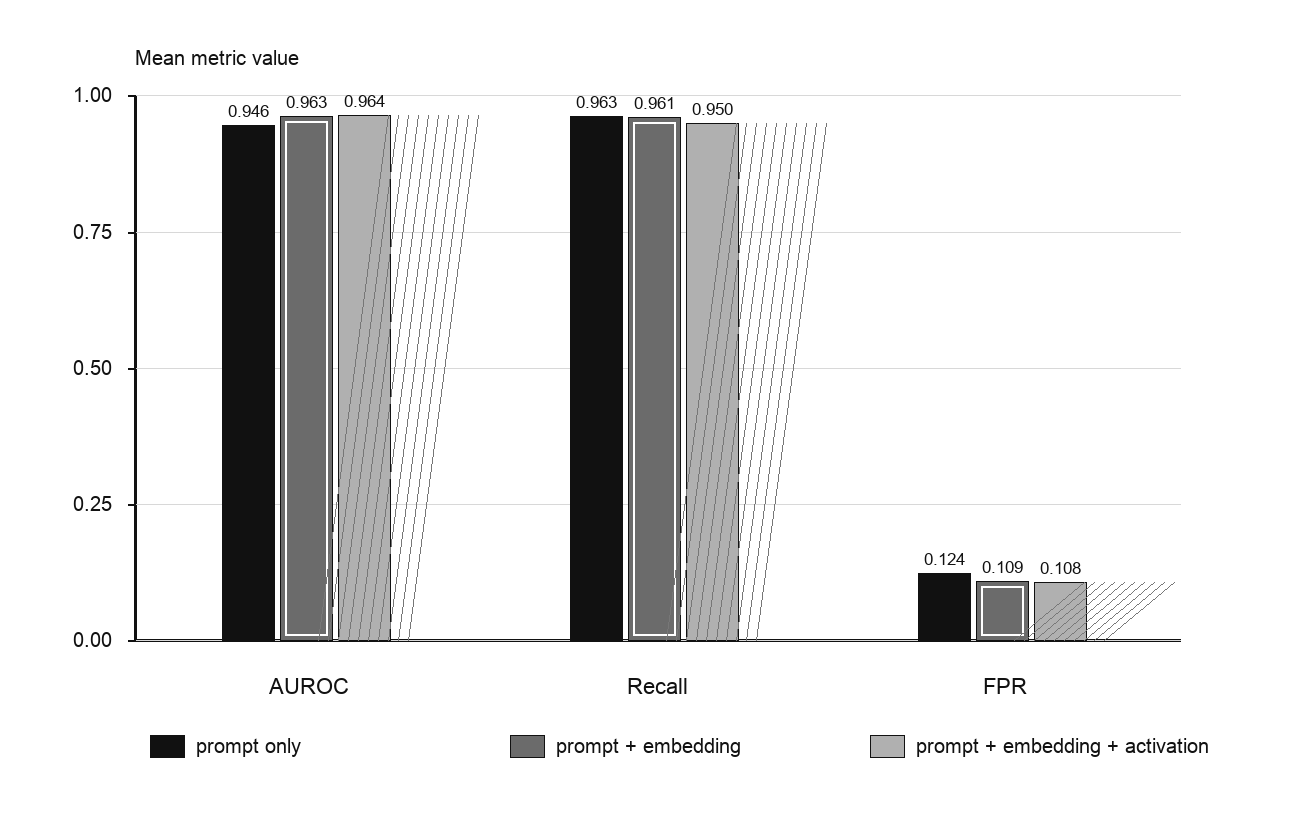
\includegraphics[width=\linewidth]{input_side_split_stability.png}
\caption{Input-side reviewed split stability under the leakage-free protocol. Prompt+embedding
improves AUROC and false-positive rate over prompt-only. Full fusion has marginally higher AUROC but
lower recall/F1, so activation remains an audit/research signal in the current policy.}
\label{fig:inputside}
\end{figure}

\begin{table}[H]
\centering
\begin{tabular}{lrrrrr}
\toprule
Condition & AUROC & Recall & FPR & FP & FN \\
\midrule
Prompt only & 0.9458 & 0.9631 & 0.1238 & 11.63 & 4.80 \\
Prompt+embedding & 0.9627 & 0.9608 & 0.1085 & 10.20 & 5.10 \\
Prompt+activation & 0.9609 & 0.9569 & 0.1195 & 11.23 & 5.60 \\
Prompt+embedding+activation & 0.9641 & 0.9500 & 0.1078 & 10.13 & 6.50 \\
\bottomrule
\end{tabular}
\caption{Input-side split-stability means over 30 deterministic reviewed-label splits. Activation
scores are leakage-free: calibration predictions are out-of-fold and holdout predictions are
out-of-split.}
\label{tab:inputside}
\end{table}

\subsection{Output Classifier}

The output classifier tests whether generated text adds evidence that prompt-side features miss. We
built a 134-row prompt/response set from reviewed prompt examples, generated responses separately,
then scored the generated response text with the same Qwen3Guard interface. This intentionally
keeps prompt risk and output risk separate: the output classifier is evaluated on model behavior,
not on the original prompt text. Table~\ref{tab:output} and Figure~\ref{fig:output} show that
output-inclusive fusion does not improve the strongest input-side result on the current response
set. We therefore retain output scoring as post-generation audit and compliance evidence, not as a
positive runtime blocking weight.

\begin{figure}[H]
\centering
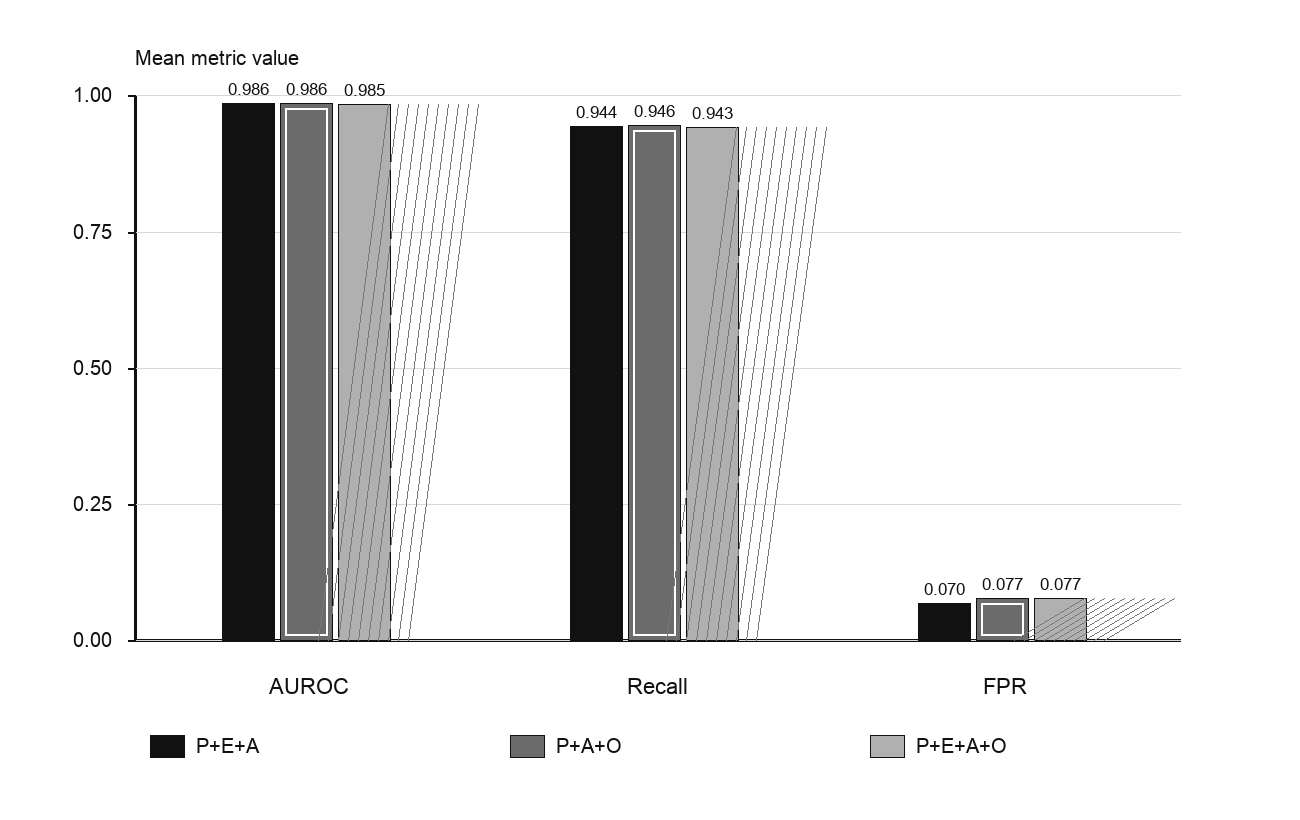
\includegraphics[width=\linewidth]{output_ablation.png}
\caption{Output-classifier ablation. Output scoring is implemented and useful for audit, but the
current prompt/response set does not justify positive runtime fusion weight.}
\label{fig:output}
\end{figure}

\begin{table}[H]
\centering
\begin{tabular}{lrrr}
\toprule
Condition & AUROC & Recall & FPR \\
\midrule
Prompt+embedding+activation & 0.9864 & 0.9443 & 0.0697 \\
Prompt+activation+output & 0.9858 & 0.9457 & 0.0773 \\
Prompt+embedding+activation+output & 0.9851 & 0.9429 & 0.0773 \\
\bottomrule
\end{tabular}
\caption{Output-inclusive calibration over 20 deterministic splits.}
\label{tab:output}
\end{table}

\subsection{Session Classifier}

The session experiments address a separate question: can multi-turn evidence catch risk missed by
single-turn scoring? We first tried mathematical accumulation over isolated turn scores; that
negative result motivated a real session classifier. We then built two representations. The compact
representation contains a safety-specific state: salient turns, domains, severity, trend,
composition cues, and evasion/operational-detail indicators. The full-transcript representation is
an oracle-like baseline that sends the role-aware transcript to the classifier. We compare both
against single-turn maximum score and against naive max fusion. R-Judge provides labeled session
metrics; MHJ is unsafe-only and is therefore used only for unsafe-recall stress.

\begin{figure}[H]
\centering
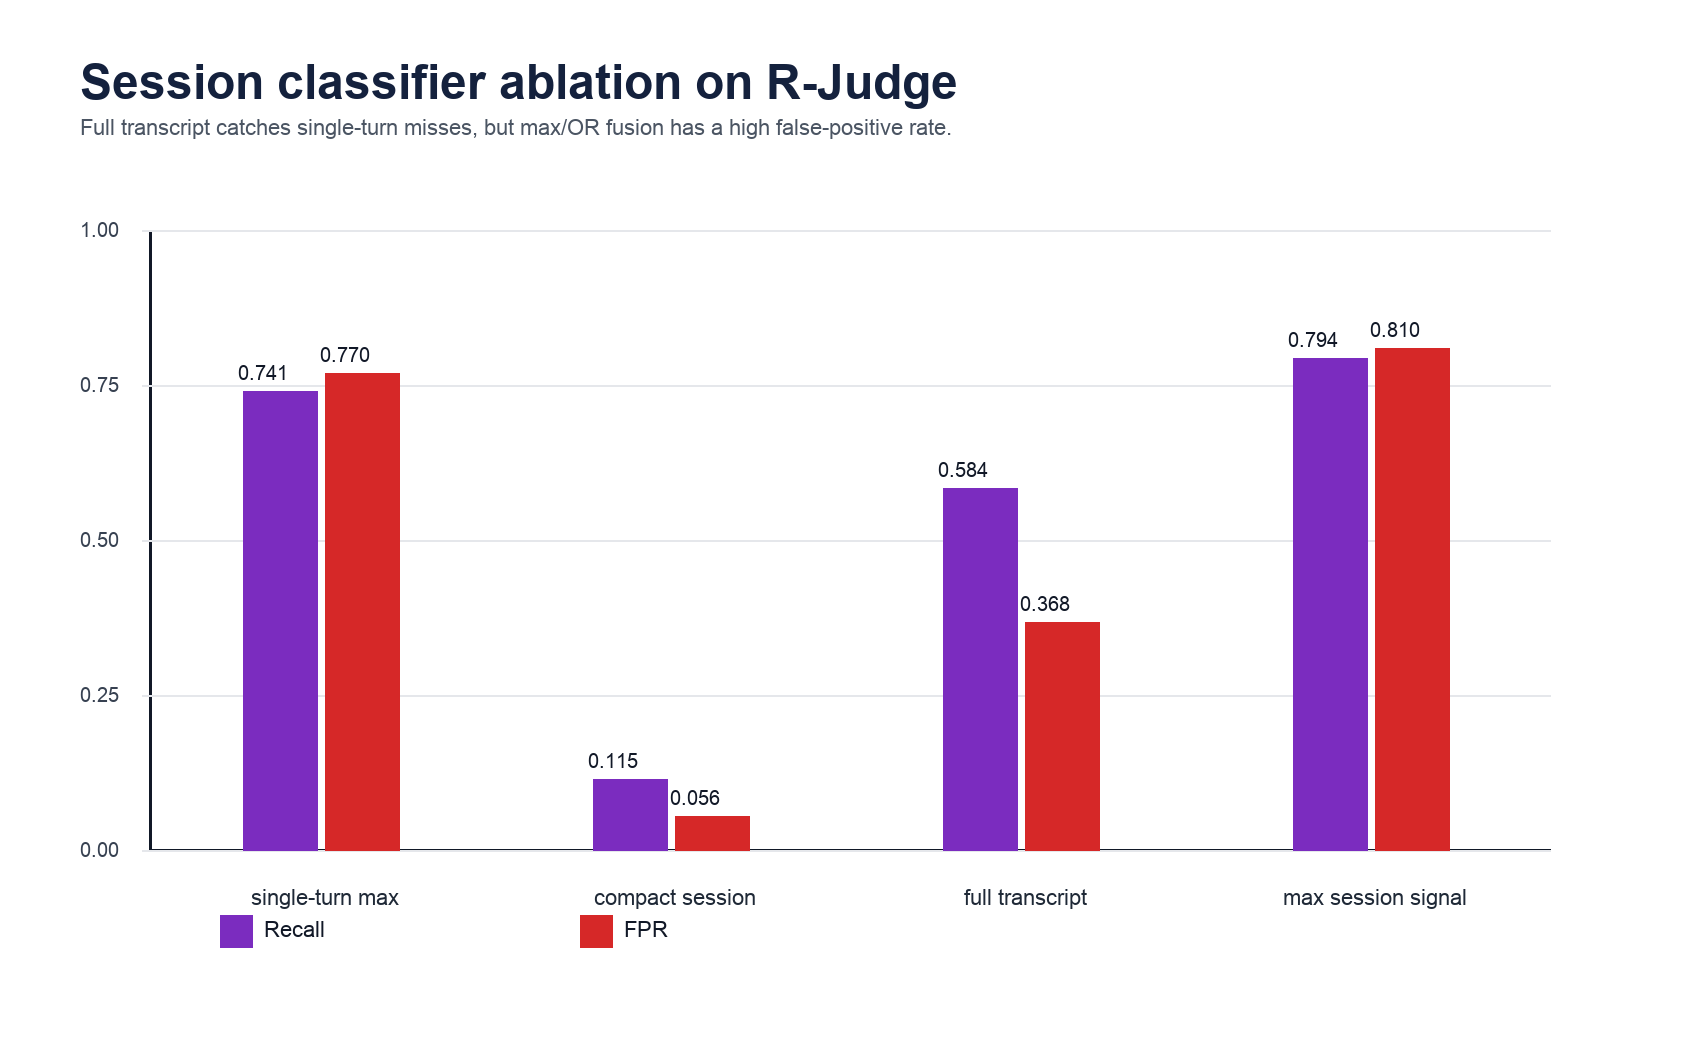
\includegraphics[width=\linewidth]{session_ablation_rjudge.png}
\caption{R-Judge session ablation. Full transcript catches single-turn misses, but naive max fusion
raises false positives. Compact state is efficient but too lossy in the current implementation.}
\label{fig:session}
\end{figure}

\begin{table}[H]
\centering
\begin{tabular}{lrrrr}
\toprule
Condition & AUROC & Recall & FPR & FNs caught \\
\midrule
Single-turn max & 0.5471 & 0.7413 & 0.7695 & 0 \\
Compact session & 0.5299 & 0.1154 & 0.0558 & 1 \\
Full transcript & 0.6105 & 0.5839 & 0.3680 & 14 \\
Max session signal & 0.5570 & 0.7937 & 0.8104 & 15 \\
\bottomrule
\end{tabular}
\caption{R-Judge session comparison at threshold 0.55. ``FNs caught'' counts unsafe sessions missed
by single-turn max but caught by the session condition.}
\label{tab:session-rjudge}
\end{table}

\begin{table}[H]
\centering
\begin{tabular}{lrr}
\toprule
Condition & Recall & Single-turn FNs caught \\
\midrule
Single-turn max & 0.7984 & 0 \\
Compact session & 0.4133 & 4 \\
Full transcript & 0.6956 & 24 \\
Max session signal & 0.8508 & 26 \\
\bottomrule
\end{tabular}
\caption{MHJ unsafe-only stress comparison at threshold 0.55. No AUROC or FPR is reported because
the current MHJ slice has no safe sessions.}
\label{tab:session-mhj}
\end{table}

\subsection{Tool/Action Gate}

The tool/action stage is included because agent systems can be safe in text while risky in proposed
actions or arguments. In the current implementation this stage is a deterministic reference gate
over tool name, action type, argument sensitivity, and permission context. It is not included in the
quantitative tables because we have not yet built a dedicated benchmark of benign and harmful
tool/action proposals. The correct current role is therefore design coverage rather than empirical
claim.

\FloatBarrier

\section{Discussion}

\paragraph{What earns runtime weight?}
The reviewed-label evidence supports prompt+embedding as the current input-side runtime core.
Embedding receives positive weight not because semantic proximity is assumed superior, but because
it improves the selected cross-fitted reviewed-label tradeoff over prompt-only.

\paragraph{What does not earn runtime weight yet?}
Activation is useful for representation research, but the leakage-free reviewed-label protocol did
not justify positive runtime weight. Output scoring is useful for post-generation audit and
compliance measurement, but the current response set does not justify positive weight. Full
transcript session scoring catches missed unsafe sessions, but naive OR/max fusion is
false-positive heavy. Compact session evidence is too lossy in its current form.

\paragraph{Negative results as contribution.}
The project would be weaker if it simply added every signal to a final score. RAMP's contribution is
the ability to evaluate each signal's role under a declared protocol. Some implemented features are
therefore deliberately assigned zero runtime weight.

\section{Limitations}

The reviewed prompt set is targeted toward hard disagreements and is not a broad deployment
distribution. Some session datasets are unsafe-only or unlabeled, limiting AUROC and FPR claims.
The activation probe is trained and evaluated on extracted GPT-OSS representations, not on a
production-serving stack. Output and session experiments are small-scale and need more human-reviewed
coverage. Tool/action gating is implemented as a reference design but lacks benchmark validation.
Finally, all thresholds and weights are research artifacts, not production safety guarantees.

\section{Reproducibility}

The repository records the frozen policies, report generator, and artifact registry. The
consolidated report is generated by:
\begin{verbatim}
python scripts/build_v0_consolidated_report.py \
  --output-md docs/reports/ramp_v0_consolidated_research_report.md
\end{verbatim}
The same script can also emit an ignored JSON summary with \texttt{--output-json}.
The paper figures are generated by:
\begin{verbatim}
python scripts/build_paper_assets.py
\end{verbatim}
The paper source, generated figures, and report artifacts are versioned in the project repository.

\section{Conclusion}

RAMP is a feature-complete research reference implementation for multi-stage safety
classification. Its current paper-grade lesson is careful and bounded: prompt+embedding is the
best-supported input-side runtime core; activation, output, and session signals add audit, research,
or escalation value but require stronger blind-holdout evidence before they become positive blocking
weights. This result
supports RAMP as a useful framework for studying cumulative safety evidence, while preserving clear
limitations around data scale, calibration, and deployment readiness.

\FloatBarrier
\bibliographystyle{plainnat}
\bibliography{references}

\end{document}
